% !TeX root = ../thuthesis-example.tex

\chapter{实验结果}
\label{result}

前述几章讨论了本研究在仿真器上的改进、在自主导航算法和训练方法上的设计以及开发的部署平台。本研究的主要创新点是提出了一种基于强化学习的自主导航算法,以及提升其效率的三段式训练方法,其它两部分内容都是为了配合该自主导航算法,使整个系统发挥出更好的性能。本章将首先展示自主导航算法和三段式训练方法在训练和仿真中展现出的优良性能,然后展示其在真机部署实验中的效果。

由于本研究是系统性的研究,因此最终性能尤其是实机部署中的性能与整个系统构建有关,例如使用何种传感器、飞行控制器等。因此在介绍有关结论时将尽可能详细介绍实验的环境以及实验的设置,并尽可能地测试每个组件单独的性能以给出参考。

\section{三段式训练方法}

三段式训练方法主要解决了原有使用深度图输入的强化学习速度慢的问题,其主要性能体现在训练速度上。本节将主要展示三段式训练方法第一、三步骤在训练过程中起到的效果,并对比三段式训练方法与使用深度图作为输入直接强化学习的训练方法在训练效率上的优势。

\subsection{预训练点云编码器}

这一训练阶段我们使用了自监督学习的方法训练了点云编码器。训练过程如\ref{pcd_encoder}节所示。训练过程中取学习超参数如表\ref{encoder_param}所示。编码器-解码器(encoder-decoder)自监督学习是通过对称结构将复杂信息编码至低维空间的方法,此过程势必会损失一些信息,而图\ref{fig_pcd_encoder_1},\ref{fig_pcd_encoder_2},\ref{fig_pcd_encoder_3}是编码器-解码器结构重建图与原图对比图,两张图相似程度表示了编码过程中信息损失情况。

\begin{figure}
  \centering
  \subcaptionbox{原点云(切片)}
    {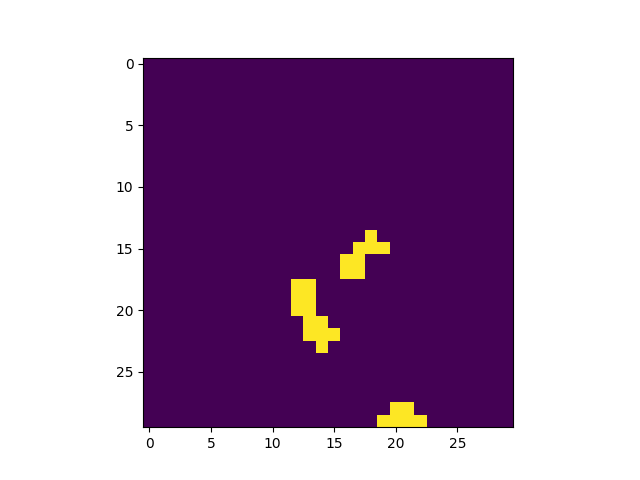
\includegraphics[width=0.47\linewidth]{encoder_2.png}}
  \subcaptionbox{重建后点云}
    {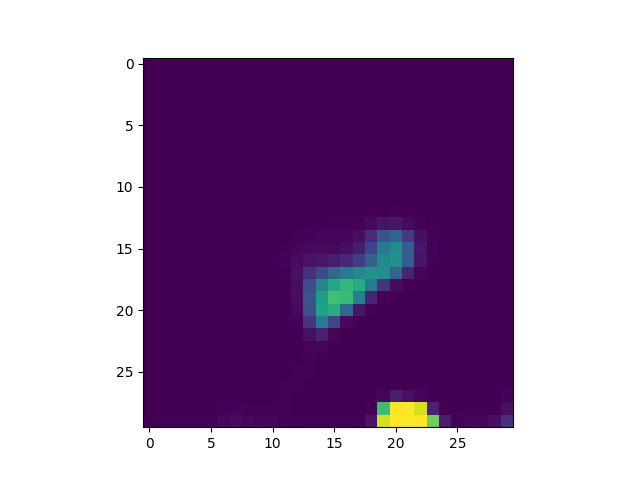
\includegraphics[width=0.47\linewidth]{encoder_2-rebuild.png}}
  \caption{点云编码器预训练效果1}
  \label{fig_pcd_encoder_1}
\end{figure}
\begin{figure}
    \centering
    \subcaptionbox{原点云(切片)}
      {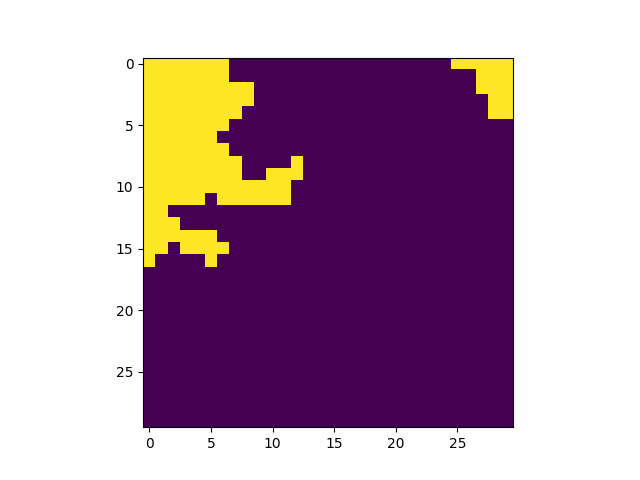
\includegraphics[width=0.47\linewidth]{encoder_5.png}}
    \subcaptionbox{重建后点云}
      {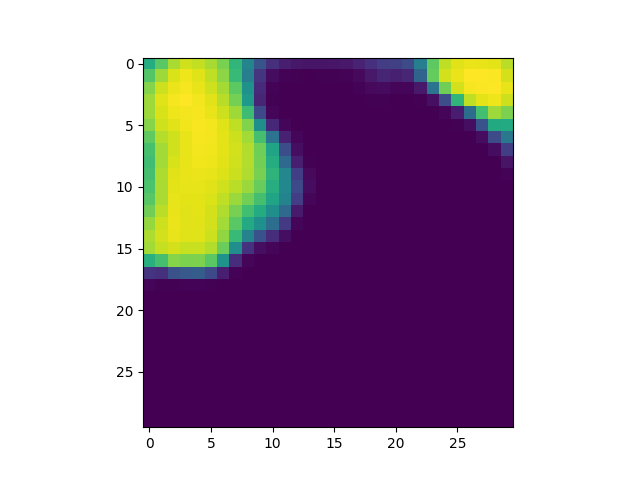
\includegraphics[width=0.47\linewidth]{encoder_5-rebuild.png}}
    \caption{点云编码器预训练效果2}
    \label{fig_pcd_encoder_2}
  \end{figure}
  \begin{figure}
    \centering
    \subcaptionbox{原点云(切片)}
      {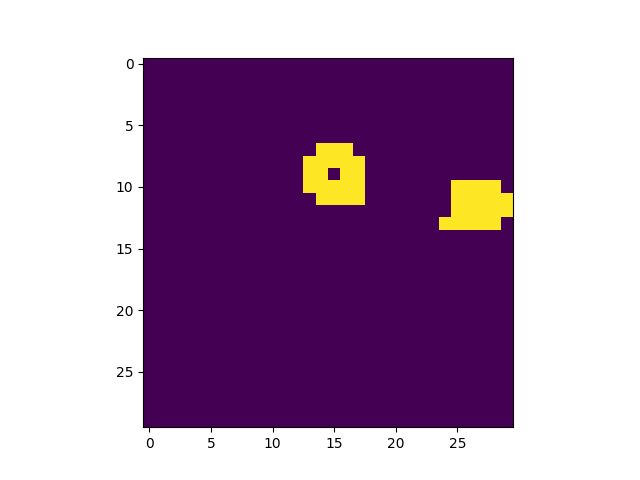
\includegraphics[width=0.47\linewidth]{encoder_6.png}}
    \subcaptionbox{重建后点云}
      {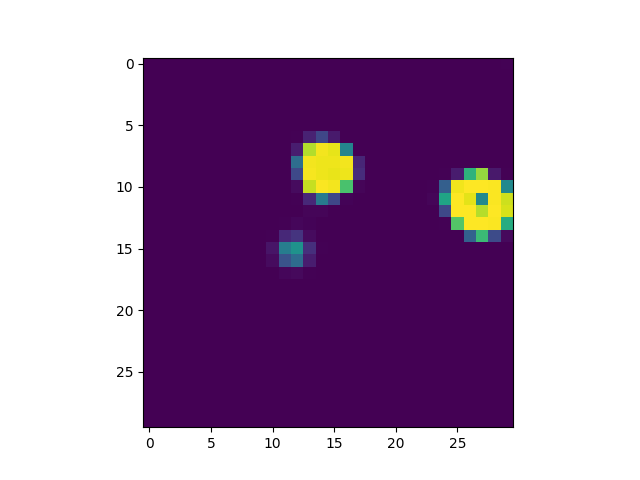
\includegraphics[width=0.47\linewidth]{encoder_6-rebuild.png}}
    \caption{点云编码器预训练效果3}
    \label{fig_pcd_encoder_3}
  \end{figure}

对比可以发现对于较稀疏的障碍(例如树林中零散的树干),该编码器基本能够重建障碍物的位置、大小情况,但对于较稠密的障碍(例如飞行至树冠位置)重建能力较差。但这并不影响正常飞行时的编码表现,因为在正常飞行时飞行器的观测基本全部是稀疏的。因此该编码器在常见的飞行场景下编码能力完全满足自主导航飞行的需求。

\subsection{编码器对齐}

本阶段使用调整后的点云编码器做监督,有监督地训练深度图编码器,训练过程如\ref{encoder_align}节所述。训练过程使用的超参数如表\ref{encoder_param}所示。

\begin{table}
    \centering
    \begin{tabular}{cccccc}
    \hline
        任务 & 学习率 & 迭代次数 & 小批次 & 训练损失函数 & 验证损失函数 \\ \hline
        预训练点云编码器 & 0.001 & 400 & 2048 & BCE & MSE \\ 
        编码器对齐 & 0.01 & 800 & 1024 & MSE & BCE \\ \hline
    \end{tabular}
    \label{encoder_param}
    \caption{预训练点云编码器和编码器对齐超参数表}
\end{table}

\subsection{三段式学习方法对效率的提升}

三段式训练方法能够大幅度提升训练整个框架的效率,表\ref{simulation_eff}展示了三段式训练方法相比于直接使用深度图作为输入的强化学习方法在训练过程中的效率提升。特别地,在算法调试的过程中预训练和编码器对齐往往需要训练的次数较少。而主要的调试对象强化学习阶段则会被训练很多次。因此从算法调试的角度,三段式训练方法将调试效率提升了1$\sim$2个数量级。

\begin{table}
    \centering
    \begin{tabular}{ccc}
    \hline
        ~ &  深度图为输入的强化学习训练 & 三段式训练方法 \\ \hline
        预训练用时 & 0 & 10min \\ 
        强化学习FPS & 60 & 1500 \\ 
        算法收敛(采集50M数据)用时 & (预计)232h & 9.5h \\ 
        编码器对齐用时 & 0 & 30min \\ 
        训练算法总耗时 & (预计)232h & 10.2h \\ 
        测试平台可同时运行实验数 & 1 & 4 \\ \hline
    \end{tabular}
    \caption{两种训练方法的训练效率}
    \label{simulation_eff}
\end{table}

\section{自主导航算法性能}

% 超参数表格
本节将主要介绍自主导航算法的性能,即强化学习训练部分。本节将首先介绍训练条件的设置,然后可视化地展现自主导航算法穿越丛林的性能,最后介绍一组消融实验以表明\ref{pcd_rl}节中提到的训练技术和预训练的点云编码器的有效性。

本研究的强化学习部分使用PPO算法,其超参数设置如表\ref{tab_rl_param}所示。特别地,相较于其它强化学习任务,自主导航任务观测空间、动作空间均较大,因此特别设置了“数据复用次数”较小(常见设置为15)、小批次数量较大(常见设置为8、16)和最大梯度较小(常见设置为10.0)以降低每次更新算法的步长,避免在训练之初由于错误的探索导致算法过快更新至错误的策略从而导致整个训练失败的问题。

\begin{table}[!ht]
    \centering
    \begin{tabular}{ccc}
    \hline
        ~ & 超参数名称 & 参数值 \\ \hline
        \multirow{4}*{环境参数} & 回合长度 & 500 \\ 
        & 回合数 & 100000 \\ 
        & 障碍物平均密度 & 1/49$\sim$1/36 \\ 
        & 飞行轨迹长度 & 10m$\sim$30m \\ 
        \multirow{6}*{PPO算法参数} & 数据复用次数 & 6 \\ 
        & 小批次数量 & 24 \\ 
        & 增益 & 0.01 \\ 
        & 学习率 & 10min \\ 
        & 折扣因子 & 0.99 \\ 
        & 最大梯度 & 6.0 \\ \hline
    \end{tabular}
    \caption{算法训练超参数}
    \label{tab_rl_param}
\end{table}

\subsection{训练效果}

我们将三段式训练中前两步训练的结果先拿来进行测试。在一片障碍物平均间距4.5m的树林中测试了自主导航算法的能力。飞行轨迹可视化如图\ref{fig_traj}所示。从图中可以发现飞行器在障碍物前约3m处开始避让障碍物,这与训练设定中深度相机和点云感知距离为3$\sim$4m相吻合。轨迹在无障碍物处较为平滑,这体现了奖励设计中$r_v,\ r_\omega$两项的作用。
\begin{figure}
    \centering
    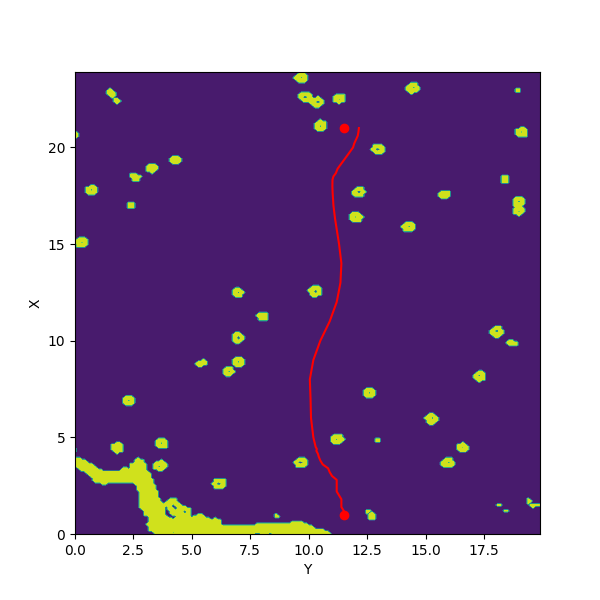
\includegraphics[width = 1\textwidth]{traj_viz.png}
    \caption{飞行轨迹可视化(俯视图)}
    \caption*{平均障碍物间距4.5m,目标距离20m,飞行速度4m/s}
    \label{fig_traj}
\end{figure}

由于训练过程中使用了域随机化的技巧,我们还测试了算法在不同速度下的性能,并与相关算法进行了对比,比较结果如表\ref{tab_generalize}所示。可以发现相比于在特定速度下训练的算法,本算法在速度这一指标上的泛化性较好。

\begin{table}
    \centering
    \begin{tabular}{ccc}
    \hline
        算法 & 3m/s速度 & 5m/s速度 \\ \hline
        Learning\cite{loquercio2021learning} & 14.3 & 19.8 \\ 
        ego planner\cite{zhou2020ego} & 20.0 & $\backslash$ \\ 
        本方法 & 17.2 & 18.2 \\ \hline
    \end{tabular}
    \caption{算法泛化性能对比}
    \caption*{在不同速度下的平均探索距离,单位m,目标点距离20m}
    \label{tab_generalize}
\end{table}

\subsection{消融实验}

消融实验(ablation experiment)是深度学习领域最常见的论证方法创新有效性的方法。其操作是删除一些模块(或用随机的模块替换一些对训练有帮助的模块)并检查算法性能的降低程度,以此来判断该模块对算法性能的贡献。本节将介绍一组消融实验以证明\ref{pcd_rl}节中提到的编码器固定和预训练的点云编码器的有效性。

本消融实验设置了三个实验组,实验组对照组情况如表\ref{tab_ab_exp}所示。实验设置了三个指标、分别是总奖励值、平均探索路径长度、平均回合长度,分别刻画算法在导航任务中的综合性能、导航探索的范围和避免碰撞保证存活的能力。

经过训练,实验结果如图\ref{fig_tot},\ref{fig_movement},\ref{fig_eps_len}所示。分析结果不难发现,without freezing encoder实验组虽然仍能学习到一定自主导航的能力,但其探索距离上限没有对照组高。而该实验组的平均回合长度与对照组相当甚至更长,说明该实验组学习到了避障方面的能力但自主导航的能力有所下降。这与我们理论分析中提到编码器固定的必要性相符。而另外两组实验则完全无法通过训练获得自主导航的能力,这是因为点云编码器的参数量相比规划器更大,训练难度也更大,如果不使用预训练直接强化学习训练,算法将难以收敛。这体现了预训练点云编码器的必要性。

\begin{table}
    \centering
    \begin{tabular}{cccc}
    \hline
        组别 & 实验名称 & 初始点云编码器 & 编码器固定  \\ \hline
        对照组 & full & 预训练 & 是  \\ 
        \multirow{3}*{实验组} & without freezing encoder & 预训练 & 否  \\ 
        & random encoder & 随机 & 是  \\ 
        & train encoder in RL & 随机 & 否  \\ \hline
    \end{tabular}
    \caption{消融实验设置}
    \label{tab_ab_exp}
\end{table}
\begin{figure}
    \centering
    \includegraphics[width = 0.9\textwidth]{tot_reward.png}
    \caption{消融实验结果:总奖励值}
    \label{fig_tot}
\end{figure}
\begin{figure}
    \centering
    \includegraphics[width = 0.9\textwidth]{move_x.png}
    \caption{消融实验结果:平均探索路径长度}
    \label{fig_movement}
\end{figure}
\begin{figure}
    \centering
    \includegraphics[width = 0.9\textwidth]{eps_len.png}
    \caption{消融实验结果:平均回合长度}
    \label{fig_eps_len}
\end{figure}
% 消融实验

\section{部署平台基本飞行性能}

% 8字飞行,PID和MPC性能差距 ROSBAG
为测试部署平台的基本飞行性能,本项目使用了8字飞行测试。其飞行轨迹为8字型线(figure-eight curve)也称为赫罗诺双纽线(lemniscate of Gerono),如图\ref{fig_8}所示。曲线方程可以表示为
\[
    x^4-x^2+y^2 = 0
\]
其参数化的表示形式(也是飞行过程中实际使用的形式)为
\[
    x = \frac{t^2-1}{t^2+1},\ y = \frac{2t(t^2-1)}{(t^2+1)^2}
\]
在测试中设置8字形轨迹长度为5m,最大飞行速度为3m/s。选择基线Baseline算法为ego-planner配套的部署平台\cite{zhou2020ego}。绘制测试过程中目标轨迹、飞行轨迹如图\ref{fig_8traj}所示。我们还记录了飞行过程中飞行器$x,\ y$方向的加速度,如图\ref{fig_acc_x},\ref{fig_acc_y}所示。分析三张图可以发现基线方法在飞行初末加减速时有偏离轨迹的情况。同时$x,\ y$两个方向上基线方法的加速度抖动幅度都明显大于本部署平台。因此本部署平台在轨迹追踪这一基础任务上的表现更好。

\begin{figure}
    \centering
    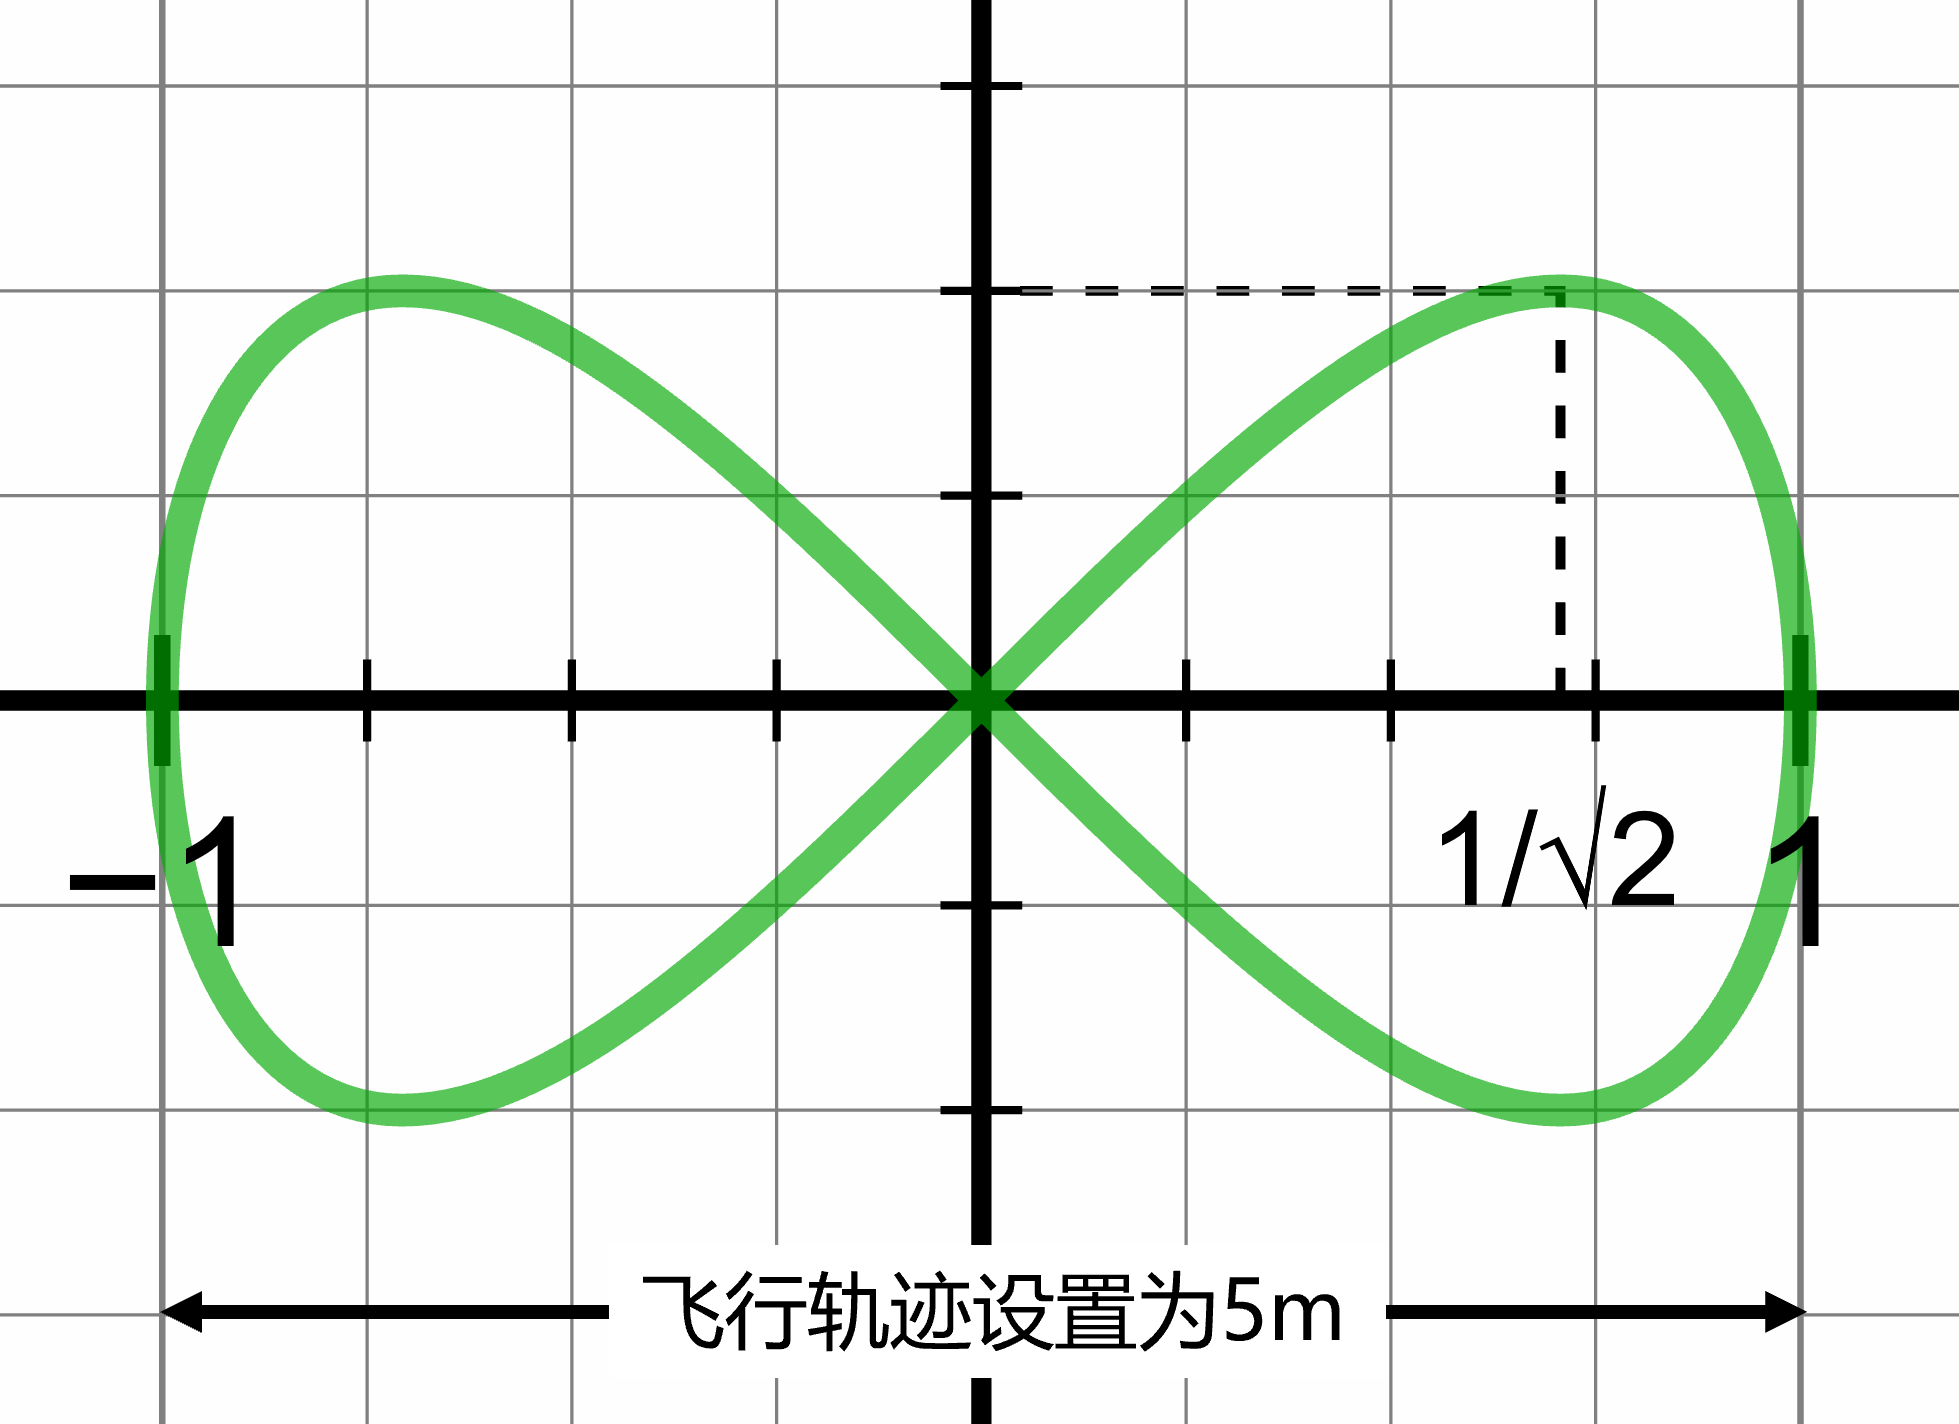
\includegraphics[width = 0.75\textwidth]{8figure.png}
    \caption{赫罗诺双纽线示意图}
    \label{fig_8}
\end{figure}
\begin{figure}
    \centering
    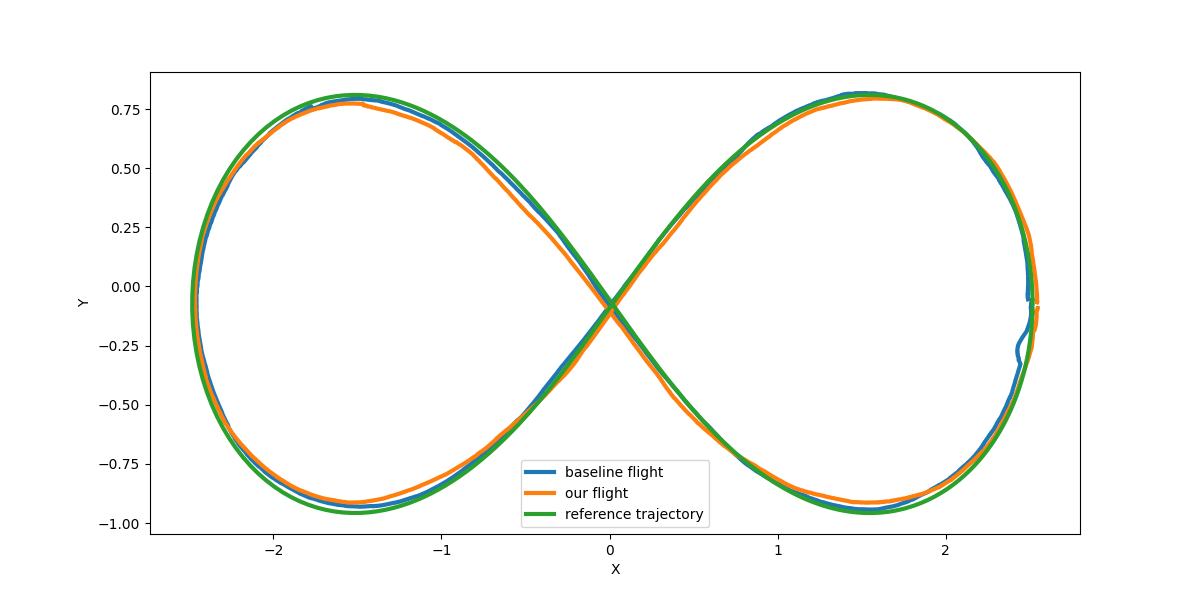
\includegraphics[width = 1\textwidth]{8figure-traj.png}
    \caption{部署平台追踪8字型轨迹}
    \label{fig_8traj}
\end{figure}
\begin{figure}
    \centering
    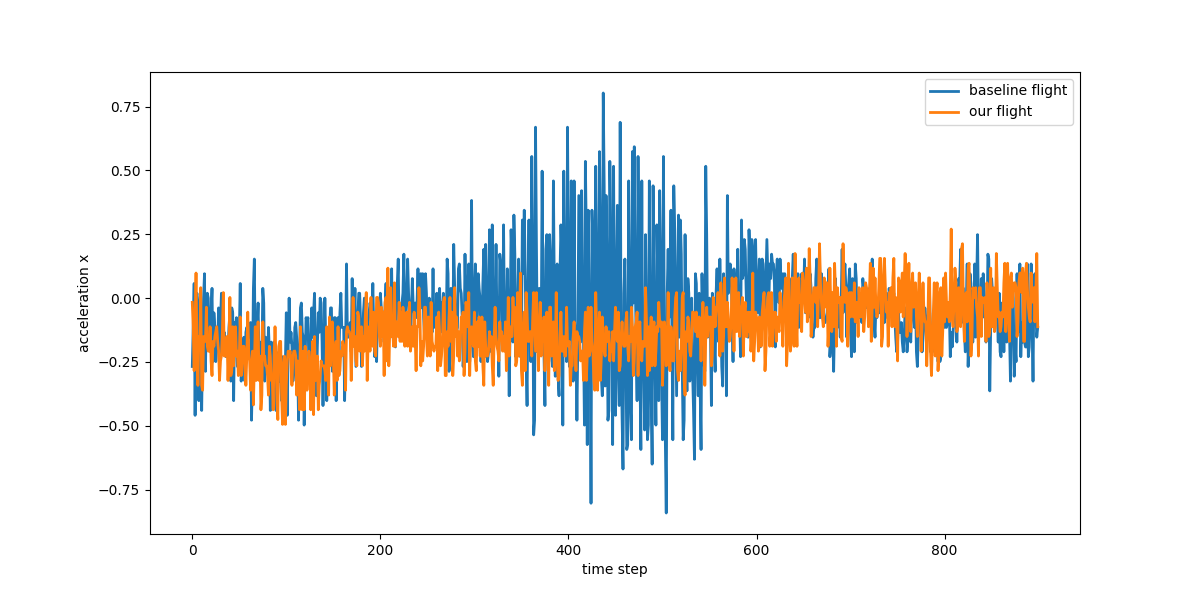
\includegraphics[width = 1\textwidth]{acc_x.png}
    \caption{追踪轨迹期间$x$方向加速度}
    \label{fig_acc_x}
\end{figure}
\begin{figure}
    \centering
    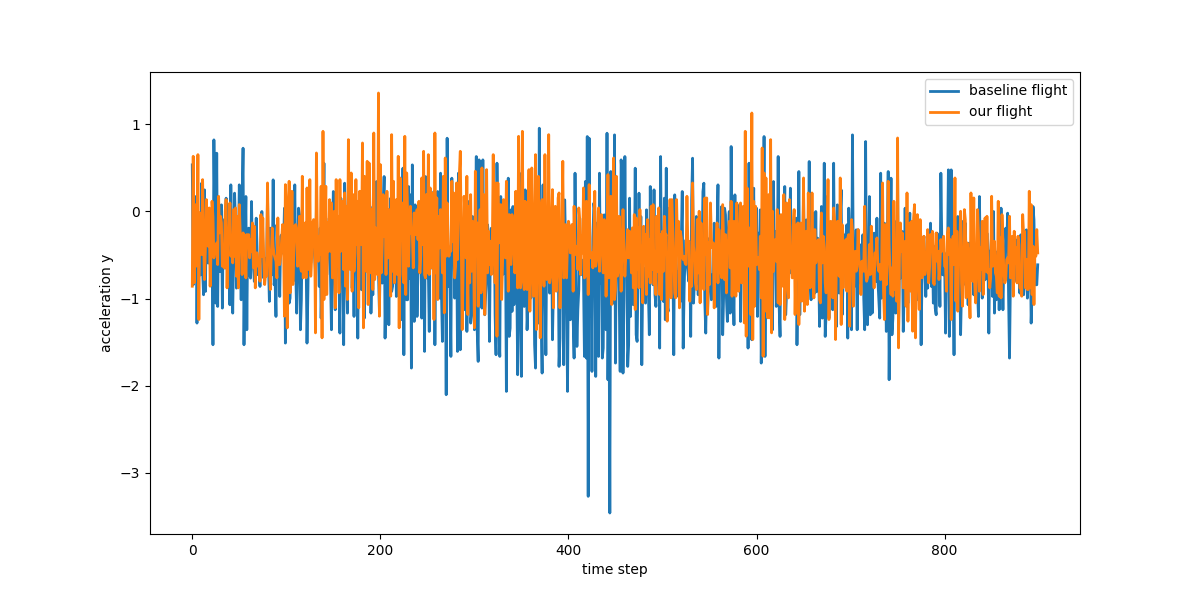
\includegraphics[width = 1\textwidth]{acc_y.png}
    \caption{追踪轨迹期间$y$方向加速度}
    \label{fig_acc_y}
\end{figure}

\section{真机算法部署}

我们将算法部署至真机,并在完成了室内场景低速情况下的导航任务的测试。测试情况如图\ref{fig_realflight}所示。。导航算法能够在室内小范围场景下完成避障导航的任务。该测试空间大小为$10m\times 10m\times 4m$,测试飞行速度为1m/s。由于时间的限制,本研究尚未完成更大测试场地和室外场景的测试。同时本研究的实机测试部分还没有定量的性能分析。这些将作为未来的工作。
\begin{figure}
  \centering
  \subcaptionbox{}
    {\includegraphics[width=0.47\linewidth]{final_1.png}}
  \subcaptionbox{}
    {\includegraphics[width=0.47\linewidth]{final_2.png}}
    \subcaptionbox{}
    {\includegraphics[width=0.47\linewidth]{final_3.png}}
    \subcaptionbox{}
    {\includegraphics[width=0.47\linewidth]{final_4.png}}
    \subcaptionbox{}
    {\includegraphics[width=0.47\linewidth]{final_5.png}}
  \caption{室内场景实机任务测试}
  \label{fig_realflight}
\end{figure}


